\documentclass[10pt,twocolumn,letterpaper]{article}

\usepackage{cvpr} \usepackage{times} \usepackage{epsfig}
\usepackage{graphicx} \usepackage{amsmath} \usepackage{amssymb}
\usepackage{subfig}

% Include other packages here, before hyperref.

% If you comment hyperref and then uncomment it, you should delete
% egpaper.aux before re-running latex.  (Or just hit 'q' on the first
% latex run, let it finish, and you should be clear).
\usepackage[pagebackref=true,breaklinks=true,letterpaper=true,colorlinks,bookmarks=false]{hyperref}


% \cvprfinalcopy % *** Uncomment this line for the final submission

\def\cvprPaperID{****} % *** Enter the 3DIMPVT Paper ID here
\def\httilde{\mbox{\tt\raisebox{-.5ex}{\symbol{126}}}}

% Pages are numbered in submission mode, and unnumbered in
% camera-ready
\ifcvprfinal\pagestyle{empty}\fi
\begin{document}

%%%%%%%%% TITLE
\title{Texture Mapping 3D Models of Indoor Environments with Noisy
  Camera Poses}

\author{First Author\\
  Institution1\\
  Institution1 address\\
  {\tt\small firstauthor@i1.org}
  % For a paper whose authors are all at the same institution, omit
  % the following lines up until the closing ``}''.  Additional
  % authors and addresses can be added with ``\and'', just like the
  % second author.  To save space, use either the email address or
  % home page, not both
  \and
  Second Author\\
  Institution2\\
  First line of institution2 address\\
  {\small\url{http://www.author.org/~second}} }

\maketitle
% \thispagestyle{empty}

%%%%%%%%% ABSTRACT
\begin{abstract}
  Automated 3D modeling of building interiors is useful in
  applications such as virtual reality and environment
  mapping. Applying textures to these models is an important step in
  generating photorealistic visualizations of data gathered by
  modeling systems.  The localization of cameras in such systems often
  suffer from inaccuracies, resulting in visible discontinuties when
  different images are projected adjacently onto a plane for
  texturing. We propose two approaches for reducing discontinuities
  during texture mapping, one to robustly accomodate images of all
  orientations, and one to take advantage of optimal situations where
  images have uniform orientation. The effectiveness of our approaches
  will be demonstrated on two indoor datasets.
\end{abstract}

%%%%%%%%% BODY TEXT
\section{Introduction}
\label{sec:introduction}
Three-dimensional modeling of indoor environments has a variety of
applications such as training and simulation for disaster management,
virtual heritage conservation, and mapping of hazardous sites. Manual
construction of these digital models can be time consuming, and as
such, automated 3D site modeling has garnered much interest in recent
years.

The aim of this paper is to present a solution for texture mapping the
3D models generated by indoor modeling systems, with specific
attention given to a human-operated system with high camera pose
errors and great variance in camera locations.

The first step in automated 3D modeling is the physical scanning of
the environment's geometry. An indoor modeling system must be able to
recover camera poses within an environment while simulatenously
reconstructing the 3D structure of the environment itself. This is
known as the simultaneous localization and mapping (SLAM) problem, and
is generally solved by taking readings from laser range scanners,
cameras, and inertial measurement units (IMUs) at multiple locations
within the environment.

Mounting such devices on a human-carried platform provides unique
advantages over vehicular-based systems in terms of agility and
portability. Unfortunately, human-operated systems also result in much
larger localization error. As a result, common methods for texture
mapping generally produce poor results, as later shown in Sections
\ref{sec:simpleTextureMapping} and
\ref{sec:existingApproaches}. Before discussing how to overcome these
challenges, we first provide an overview of the backpack modeling
system from which our test data has been obtained.

Our backpack-mounted modeling system contains five 2D laser range
scanners, two cameras, and an orientation sensor. The laser scanners
are mounted orthogonally and have a 30-meter range and a 270$^{\circ}$
field of view. The two cameras are equipped with fisheye lenses,
reaching an approximately 180$^{\circ}$ field of view, and are mounted
with one facing left and the other facing right. These cameras take
images at the rate of 5 Hz. The orientation sensor provides
orientation parameters at a rate of 180 Hz.

With the laser scanners active, the human operator wearing the
backpack takes great care to walk a path such that every wall in the
desired indoor environment is traversed and scanned lengthwise at
least once.

Using data gathered by the onboard sensors and multiple localization
and loop-closure algorithms, the backpack is first localized over its
data collection period, and a 3D point cloud of the surrounding
environment is constructed based on the laser scanner readings
relative to the backpack \cite{chen2010indoor, kua2012loopclosure, liu2010indoor}. Approximate normal vectors for each point in
the point cloud are then calculated by gathering neighboring points
within a small radius and processing them through principal component
analysis. These normal vectors allow for the classification and
grouping of adjacent points into structures such as walls, ceilings,
floors, and staircases. A RANSAC algorithm is then employed to fit
polygonal planes to these structured groupings of points, resulting in
a fully planar model \cite{sanchez2012point}. This model, consisting
of multiple 2D polygonal planes in 3D space, along with the set of
images captured by the backpack's camera, can be considered the input
to our texture mapping problem.

The remainder of the paper is organized as follows. Section
\ref{sec:simpleTextureMapping} describes the general problem of
texture mapping and examines two simple mapping approaches and their
shortcomings.  Section \ref{sec:existingApproaches} demonstrates two
previous attempts at localization refinement, and demonstrates their
inadequacies for our datasets.  Section \ref{sec:proposedApproach}
presents our proposed approach to texture mapping, combining an
improved localization refinement process with two image selection
approaches. Section \ref{sec:resultsAndConclusions} contains results
and conclusions.



\section{Simple Texture Mapping}
\label{sec:simpleTextureMapping}
\begin{figure}
  \centering
  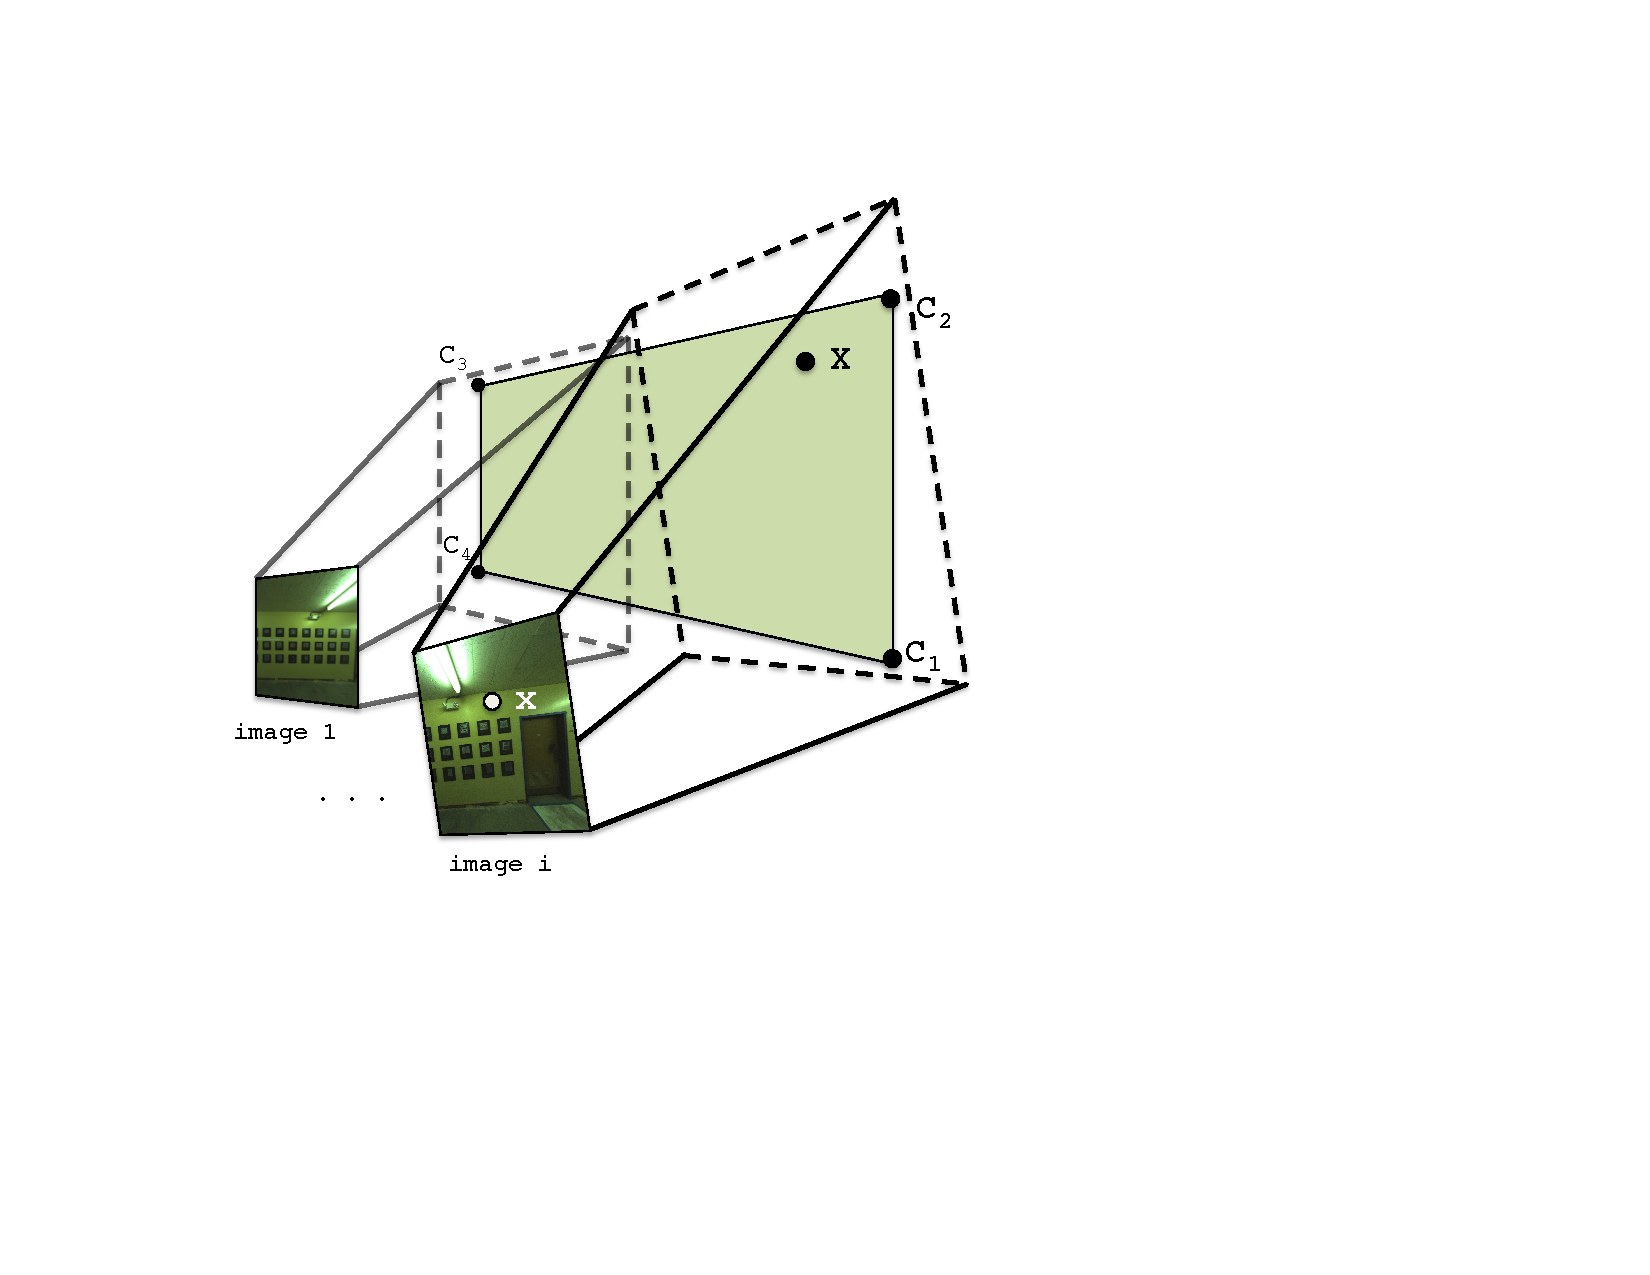
\includegraphics[height=2in]{Projection.pdf}
  \caption{Planes are specified in 3D space by four corners $C_1$ to
    $C_4$. Images are related to each plane through the camera
    matrices $P_{1..M}$. }
  \label{fig:projection}
\end{figure}

In all subsequent sections, we discuss the process of texture
mapping a single plane, as the texturing of each of our planes is
independent and can be completed in parallel.

The geometry of the texture mapping process for a plane is shown in
Figure \ref{fig:projection}.  As described earlier, we
are provided with a set of $M$ images with which we must texture our
target plane. Each image has a camera matrix $P_i$ for $i=1..M$, which
translates a 3D point in the world coordinate system to a 2D point or
pixel in image $i$'s coordinates. If the 3D world point is not
contained in the image, the 2D point will simply be outside of the
image boundaries. A camera matrix $P_i$ is composed of the camera's
intrinsic parameters, such as focal length and image center, as well
as extrinsic parameters which specify the rotation and translation of
the camera's position in 3D world coordinates at the time that image
$i$ is taken. These extrinsic parameters are determined by the
backpack hardware and localization algorithms mentioned earlier. A point $X$ on the plane in 3D space
can be related to its corresponding pixel $x$ in image $i$ through the
following equation:

\[
x=project(P_iX)
\]

where
\[X = \begin{pmatrix} x \\ y \\ z \end{pmatrix} \textrm{ and }
project(X) = \begin{pmatrix} x/z \\ y/z \end{pmatrix}
\]

For the sake of simplicity, we treat all planes as rectangles by
generating minimum bounding boxes for them. Since our final textures
are stored as standard rectangular images anyway, we can simply
leave the area between plane boundary and bounding box untextured, or
crop it out as needed. A plane to be textured is thus defined by a
bounding box with corners $C_i$ in world coordinates and a normal
vector indicating the front facing side of the plane. Our goal is to
texture this plane using images captured by the backpack, while
eliminating any visual discontinuities or seams that would suggest
that the plane's texture is not composed of a single continuous
image.

\subsection{Direct Mapping}
\label{sec:directMapping}

Ignoring the fact that the camera matrices $P_{1..M}$ are inaccurate,
we can texture the plane by discretizing it into small square tiles,
generally about 5 pixels across, and choosing an image to texture each
tile with. We choose to work with rectangular units to ensure that
borders between any two distinct images in our final texture are
either horizontal or vertical. Since most environmental features
inside buildings are horizontal or vertical, any seams in our texture
intersect them miniimally and are likely to be less noticeable.

In order to select an image for texturing tile $t$, we must first
gather a list of candidate images that contain all four of its
corners, which we can quickly check by projecting $t$ into each image
using the projection method above. Furthermore, each candidate image
must have been taken at a time when its camera had a clear
line-of-sight to $t$, which can be calculated using standard
ray-polygon intersection tests between the camera location, the center
of $t$, and other planes, all in world coordinates.

Once we have a list of candidate images for $t$, we must define a
scoring function in order to compare images and objectively select the
best one. Since camera localization errors compound over distance, we
wish to minimize the distance between cameras used for texturing and
our plane. Additionally, we desire images that are projected
perpendicularly onto the plane, maximizing the resolution and amount
of useful texture available in their projections.

These two criteria can be met by maximizing the function

\[
\frac{1}{d} \cdot (-1 \cdot C) \cdot N
\]

which minimizes camera angle $\alpha$ and distance $d$ as shown in Figure \ref{fig:scoringFunction}. 

\begin{figure}
  \centering
  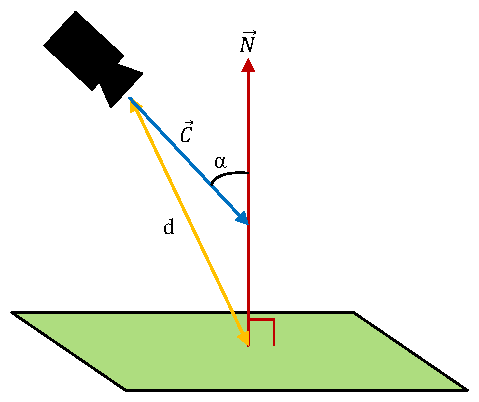
\includegraphics[height=1.5in]{scoringFunction.pdf}
  \caption{Images are selected by minimizing camera angle $\alpha$ and distance $d$.}
  \label{fig:scoringFunction}
\end{figure}



\begin{figure}
  \centering
  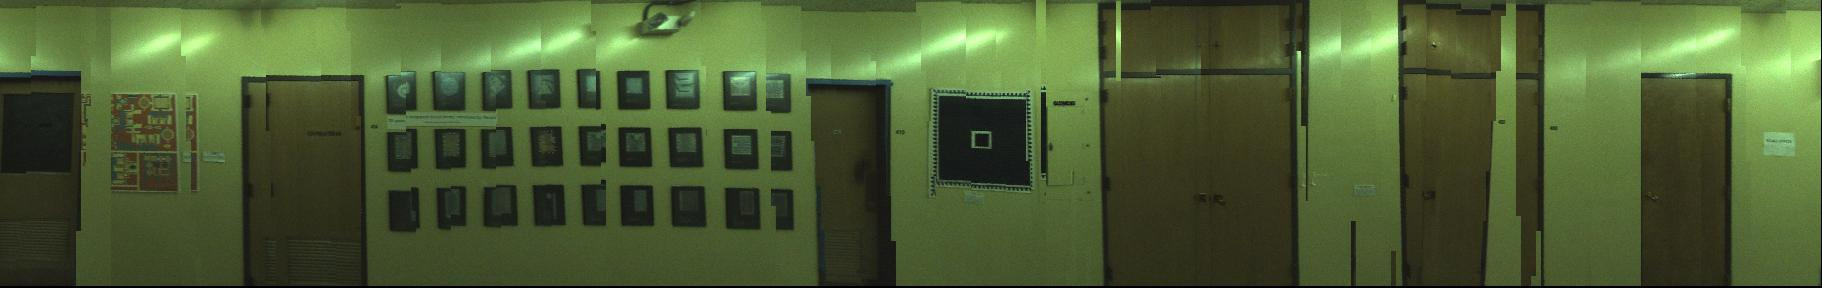
\includegraphics[width=3in]{wall1_naive.jpg}
  \caption{The result of direct texture mapping based on locally
    optimized textures.}
  \label{fig:directMapping}
\end{figure}


As Figure \ref{fig:directMapping} demonstrates, this approach leads to
the best texture for each tile independently, but overall results in
many image boundaries with abrupt discontinuities, due to significant
misalignment between images.

\subsection{Mapping with Caching}
\label{sec:mappingWithCaching}
Since discontinuities occur where adjacent tiles select different
images that do not align, it makes sense to take into account image
selections made by neighboring tiles while selecting the best image
for a given tile. By using the same image across tile boundaries, we
eliminate the discontinuity altogether. If a tile is not visible in
images chosen by its neighbors, using similar images is likely to
result in less noticeable discontinuities.

Similar to a caching mechanism, we select the best image for a tile
$t$ by searching through two subsets of images for a good candidate,
before searching through the entire set. The first subset of images is
those selected by adjacent tiles that have already been textured. We
must first check which images can map to $t$, and then of those, we
make a choice according to the same scoring function in Figure
\ref{fig:scoringFunction}. Rather than blindly reusing this image, we
ensure it meets a threshold, which we set to $\alpha < 45^\circ$, to
be considered a good image.

If no good image is found, we then check our second subset of images,
which consists of images that were taken near the images in the first
subset, both spatially and temporally. These images are not the same
as the ones used for neighboring tiles, but they were taken at a
similar location and time, suggesting that their localization and
projection are very similar. Again, if no good image is found
according to the same threshold, we then must search the entire set of
candidate images.

\begin{figure}
  \centering
  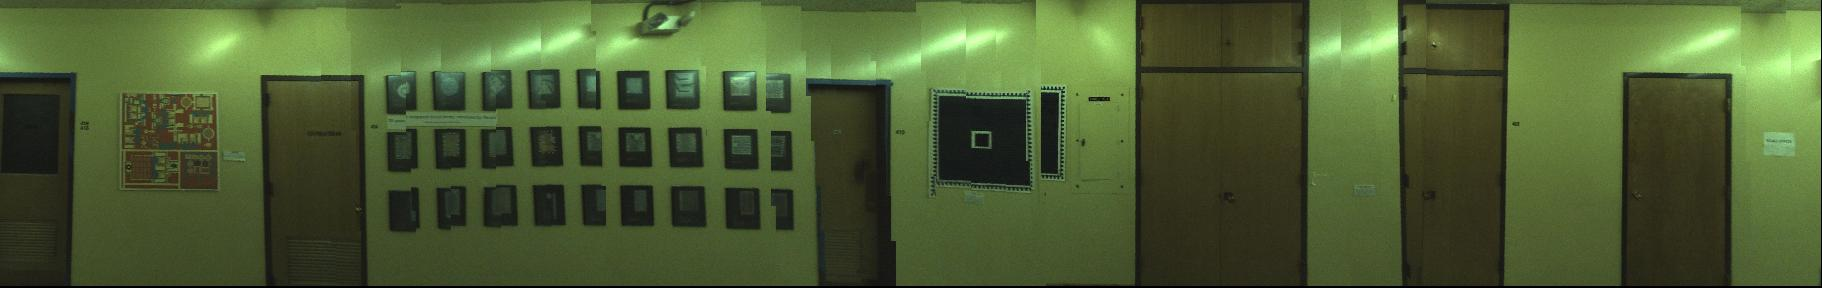
\includegraphics[width=3in]{wall1_cache_full.jpg}
  \caption{The result of adding a caching system to locally optimized
    textures.}
  \label{fig:caching}
\end{figure}


The result of this caching approach is shown in figure
\ref{fig:caching}. As compared to \ref{fig:directMapping},
discontinuities have been reduced overall, but the amount of remaining
seams suggests that image selection alone cannot produce seamless
textures. Camera matrices, or the image projections themselves have to
be adjusted in order to reliably generate clean textures.

\section{Existing Approaches to Image-Aligned Texture Mapping}
\label{sec:existingApproaches}
In order to produce seamless texture mapping, either camera matrices
need to be refined such that their localization is pixel accurate,
resulting in a perfect mapping, or image stitching techniques need to
be applied to provide this illusion. Before examining these
approaches, we first obtain a set of images to work with.

Rather than perform camera or image adjustments across the many
thousands of images acquired in a typical data collection, we opt to
work with the more limited set of images corresponding to those chosen
by the direct mapping approach, without caching. This set of images
constitutes a good candidate set for generating a final seamless
texture since it meets three important criteria. First, it contains at least one image that covers each tile on our
plane; this ensures no holes in our final texture. Second, since
images are all selected according to the same scoring function in
Figure \ref{fig:scoringFunction}, they are taken at as much of a head-on angle as possible and should project
onto the plane in similar ways. Third, as a side result of the scoring
function, selected images are only good candidates for the tiles near
their center of projection. Thus, there should be plenty of overlap
between selected images, allowing for some degree of shifting without
resulting in holes, as well as area for blending between them. With
this set of images, we now review two existing approaches towards refining and
combining their projections.

\subsection{Image Mosaicing}
\label{sec:imageMosaicing}
\begin{figure}
  \centering
  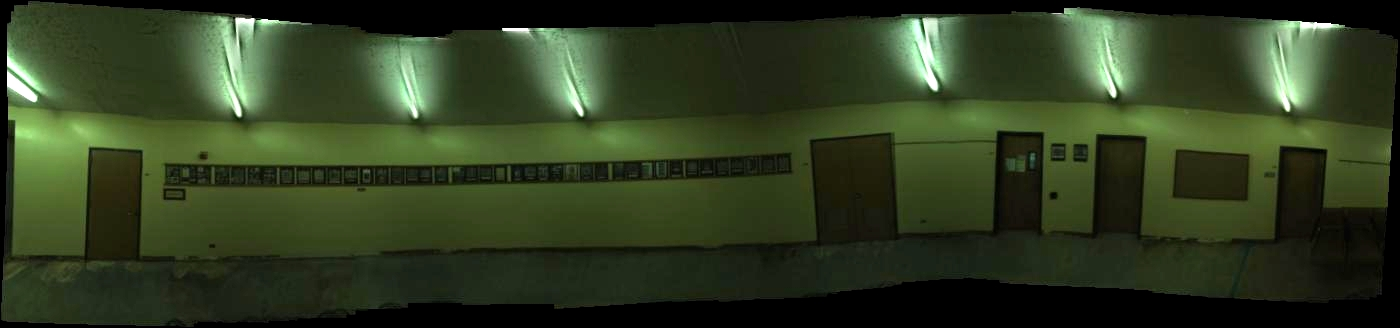
\includegraphics[width=3in]{panoMy.jpg}
  \caption{Image mosaicing. }
  \label{fig:mosaic}
\end{figure}


When images of a plane are taken from arbitrary overlapping positions,
they are related by homography \cite{hz}. Thus, existing
homography-based image mosaicing algorithms are applicable
\cite{brown2007automatic}. However, errors can compound when long
chains of images are mosaiced together using these approaches. For
example, a pixel in the $n$th image in the chain must be translated
into the first image's coordinates by multiplying by the $3\times3$
matrix $H_1 H_2 H_3 ... H_n$. Any error in one of these homography
matrices is propagated to all further images until the chain is
broken. For some chains of images this can happen almost immediately
due to erroneous correspondence matches and the resulting image mosaic
is grossly misshapen.

Figure \ref{fig:mosaic} shows the output of the AutoStitch software
package which does homography-based image mosaicing. This plane is
nearly a best-case scenerio with many features spread uniformly across
it. Even so, the mosaicing produces errors that causes straight lines
to appear as waves on the plane. This image was generated after
careful hand tuning as well. Many planes that had fewer features
simply failed outright. Thus, image mosaicing is not a robust enough
solution for reliably texture mapping our dataset.

\subsection{Image-Based 3D Localization Refinement}
\label{sec:imageBased3DRefinement}
\begin{figure}
  \centering
  
\includegraphics[width=3in]{Graph_crop.pdf}
  \caption{The graph-based localization refinement algorithm from [11]
    suffers from the problem of compounding errors. }
  \label{fig:graph}
\end{figure}

Another approach is to refine the camera matrices using image
correspondences to guide the process. Each image's camera matrix has 6
degrees of freedom that can be adjusted. Previous work on this problem
attempted to refine camera matrices by solving a non-linear
optimization problem \cite{liu2010indoor}. This process is specific to
the backpack system which generated our dataset, as it must be run
during backpack
localization\cite{liu2010indoor,chen2010indoor}. Unfortunately, this
approach suffers from a similar error propagation problem shown in
Figure \ref{fig:graph}.

\section{Proposed Method for Seamless Texture Mapping}
\label{sec:proposedApproach}
Our proposed approach towards texture mapping is a two-step
process. First, with the same input set of images as described in
Section \ref{sec:existingApproaches}, we perform image rotation and
shifting in order to maximize SIFT feature matches between images. We
then project these images onto our plane, applying textures either
with the tile caching method from Section
\ref{sec:mappingWithCaching}, or with the more specialized method
described in Section \ref{sec:seamMinimization}.

\subsection{Image Projection and Rotation}
\label{sec:projectionAndRotation}
Our localization approach begins with the projection of all our images
onto separate copies of our plane, such that no projected data is
covered up and lost. This is done in the same way as the approaches in
Section \ref{sec:simpleTextureMapping}. We then perform rotations on
these projections, as adjacent images with different orientations will
result in strong discontinuities.

These rotations are accomplished by using Hough transforms, which
detect the presence and orientation of linear features in our
images. Rather than match the orientation of such features in each
image, we simply apply rotations such that the strongest near-vertical
features are made completely vertical. This is effective for indoor
models, since strong features in indoor scenes usually consist of
parallel vertical lines corresponding to doors, wall panels,
rectangular frames, etc. If features in the environment are not
vertical, or are not parallel to eachother, this step is skipped.


\begin{figure}
  \centering
  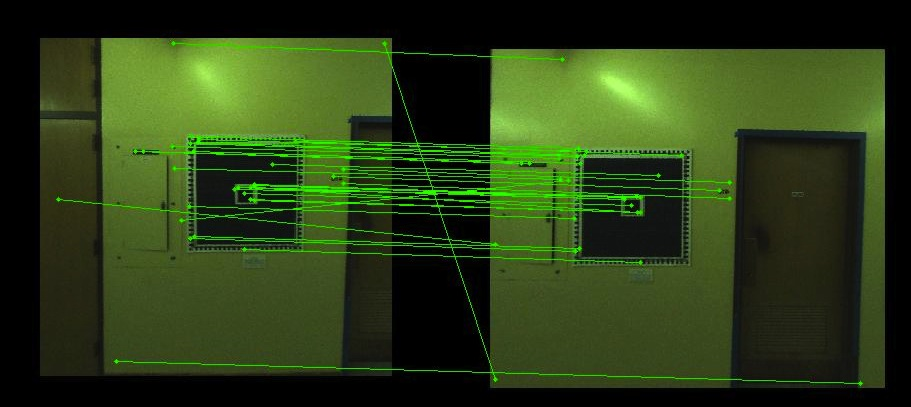
\includegraphics[width=3in]{matches.jpg}
  \caption{SIFT feature matches between overlapping images.}
  \label{fig:matches}
\end{figure}



\subsection{Robust SIFT Feature Matching using RANSAC}
\label{sec:robustSIFTFeatureMatching}
Our next step is to fix misalignment between overlapping images. We do
this by first searching for corresponding points between all pairs of
overlapping images using SIFT feature matching
\cite{lowe1999object}. An illustration of this is given in Figure
\ref{fig:matches}. The SIFT matches allow us to determine $dx$ and
$dy$ distances between each pair of features for two images on the
plane, determining where they should be projected relative to
eachother.

Since indoor environments often contain repetitive features such as
floor tiles or doors, we need to ensure that our SIFT-based distances
are reliable. In order to mitigate the effect of incorrect matches and
outliers, the RANSAC framework \cite{fischler1981random} is used for a
robust estimate of the optimal $dx$ and $dy$ distances between two
images. The RANSAC framework handles the consensus-building machinery,
and requires a fitting function and a distance function. For this
application, the fitting function simply finds the average distance
between matches in a pair of images. Our distance function for a pair
of points is the difference between those points' SIFT match distance
and the average distance computed by the fitting function; we use a 10
pixel outlier threshold. This means that a SIFT match is labeled as an
outlier if its horizontal or vertical distance is not within 10 pixels
of the average distance computed by the fitting function.

\subsubsection{Refining Image Positions using Least Squares}
\label{sec:refiningImagePositions}
There are a total of $M^{2}$ possible pairs of images, though we only
generate distances between images that overlap at SIFT feature
points. Given these distances and the original image location
estimates, we can solve a least squares problem ($\textrm{min}_{\vec{\beta}}
||X \vec{\beta} - \vec{\gamma}||_2^2 $) to estimate the correct location of the images
on the plane. The $M$-dimensional vector $\vec{\beta}$ represents the unknown $x$
and $y$ locations of each image on the plane from $1 \dots M$. The
optimal $x$ and $y$ locations are obtained in the same way, so we
only consider the $x$ locations here:

% Draw least squares problem here.

\[\vec{\beta} =
\begin{pmatrix}
  x_1, & x_2, & x_3, & \cdots & x_{M-1}, & x_M
\end{pmatrix}
\]

The $N$ by $(M+1)$ dimensional matrix $X$ is constructed with one row for each pair of images
with measured distances produced by the SIFT matching stage. A row in
the matrix has a $-1$ and $1$ in the columns corresponding to the two
images in the pair. For example, the matrix below indicates that we
generated a SIFT-based distance between images 1 and 2, images 1 and
3, images 2 and 3, etc.

\[
X =
\begin{pmatrix}
  -1 & 1 & 0 & \cdots & 0 & 0\\
  -1 & 0 & 1 & \cdots & 0 & 0\\
  0 & -1 & 1 & \cdots & 0 & 0\\
  \vdots  & \vdots & \vdots & \ddots & \vdots  & \vdots\\
  0 & 0 & 0 & \cdots & 1 & 0 \\
  0 & 0 & 0 & \cdots & -1 & 1 \\
  1 & 0 & 0 & \cdots & 0 & 0 \\
\end{pmatrix}
\]

If only relative distances between images are included then there is
no way to determine the absolute location of any of the images and the
matrix becomes rank deficient. To fix this we choose the first image
to serve as the anchor for the rest, meaning all the absolute
distances are based on its original location. This is done by adding a
row with a $1$ in the first column and the rest zeros.

Finally, the $N$-dimensional observation vector $\vec{\gamma}$ is constructed using the
SIFT-based distances generated earlier in the matching stage. The
distances are denoted as $d_1 \dots d_N$ for $N$ SIFT-based
distances. The last element in the observation vector is the location
of the first image determined by its original noisy localization, from \cite{chen2010indoor, liu2010indoor}:

\[
\vec{y}^T =
\begin{pmatrix}
  d_{1,2}, &d_{1,3}, &d_{2,3}, &\hdots &d_{N-2,N-1}, &d_{N-1,N}, &x_1
\end{pmatrix}
\]

The $\vec{\beta}$ that minimizes $||X \vec{\beta} - \vec{\gamma}||_2^2$ results in a set of
image locations on the plane that best honors all the SIFT-based
distance measurements between images. In practice there are often
cases where there is a break in the chain of images, meaning that no
SIFT matches were found between one segment of the plane and
another. In this case we add rows to the $X$ matrix and observations
to the $\vec{\gamma}$ vector that contain the original noisy $x$ and $y$ distance
estimates generated by the localization algorithm \cite{chen2010indoor, liu2010indoor}. Another way to do
this is to add rows for all neighboring pairs of images and solve a
weighted least squares problem where the SIFT distances are given a
higher weight i.e. 1, and the noisy distances generated by the localization
algorithm \cite{chen2010indoor, liu2010indoor} are given a smaller weight i.e. 0.01.

After completing this same process for the $y$ dimension as well, and
making the resultant shifts, our image projections should overlap and
match eachother with far greater accuracy.

\subsection{Relocalized Mapping with Caching}
\label{sec:mappingCachingLocalized}
Now that our images have been relocalized for much greater accuracy
relative to eachother, we can revisit the cached mapping approach from
section \ref{sec:mappingWithCaching}.  In figure \ref{fig:shifted}, we
see the wall from section \ref{sec:mappingWithCaching}, texture mapped
using the same caching method after our localization refinement
process.

\begin{figure}
  \centering
  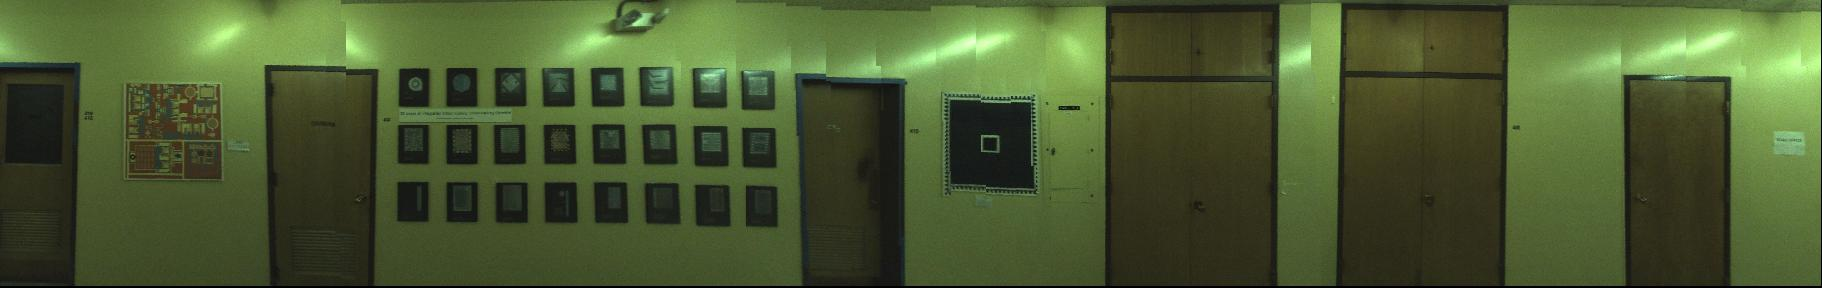
\includegraphics[width=3in]{wall1_cache_full_shifted.jpg}
  \caption{Localization refinement results in signifcantly fewer
    discontinuities in the final texture.}
  \label{fig:shifted}
\end{figure}


It should be evident that our localization adjustments resulted in a
major improvement. A great strength of our tiling approach for image
selection is that it extracts the areas with good camera angles from
each image, and thus can handle images of all types. As demonstrated
on the floor plane in figure \ref{fig:floor_suboptimal}, we can run
this process even with extremely poor image projections, where the
amount of quality texture for each image is limited. Additionally,
since our plane is discretized, we can handle arbitrarily complex
plane geometry as well.

\begin{figure}
  \centering
  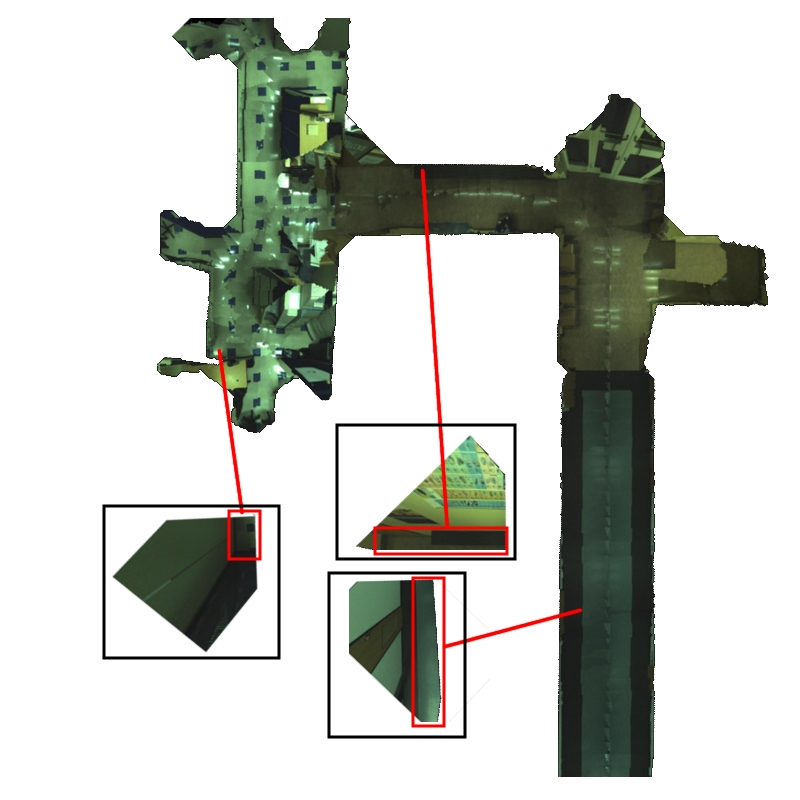
\includegraphics[width=3in]{floor_suboptimal.jpg}
  \caption{The tiling method ensures that only the most optimal
    portions of each image are used. This allows it to successfully
    handle all manner of plane and image geometry, as shown in this
    floor texture.}
  \label{fig:floor_suboptimal}
\end{figure}

Given that the backpack system's hardware and the data collection
process strive for optimal wall texturing however, we can aim for a
less conservative approach when texturing walls, and simply fall back
to this more robust approach as needed.

\subsection{Texture Mapping with Seam Minimization}
\label{sec:seamMinimization}
Since we now have higher confidence in the quality of image
boundaries, we explore an alternate method for texture mapping that
greatly reduces seams in cases where we have an abundance of optimal
images.  The cached tile approach used previously selected images
based on individual and neighboring quality of image selections, in an
effort to reduce seams between tiles. In a more optimal case, as the
backpack system provides for walls, images are all taken from close
distances and have near-rectangular projections and thus less
deviation between scores according to the scoring function in figure
\ref{fig:scoringFunction}. Thus, we can reason that rather than
selecting the set of best images, since all images are near in
quality, we should instead select the best set of images, such that
the selection together results in the cleanest final texture. We will
accomplish this by using entire images where possible, defining a cost
function between images, and seeking to minimize total cost.

\subsection{Occlusion Masking}
\label{sec:occlusionMasking}
Before we proceed with this approach, we need to ensure that our
images contain only content that should be mapped onto the target
plane in question. The tiling approach used previously checked
occlusion for each tile as it was being textured, but we plan on using
entire images, so we need to perform occlusion checks over the
entirety of each image, so we know which areas are available for
texture mapping.

Fortunately, by virtue of our indoor environments, the vast majority
of surface geometry is either horizontal or vertical, with high
amounts of right angles. This means that after masking out occluded
areas, our image projections will remain largely rectangular. We can
thus be efficient by recursively splitting each image into rectangular
pieces, and performing the same occlusion checks used in the tiling
process where needed. To actually occlude out rectangles, we simply
remove their texture, as we will ensure that untextured areas are
never chosen for texture mapping.

\subsection{Inter-Image Cost Functions}
\label{sec:interImageCosts}
In order to objectively decide which set of images results in the
cleanest texture, we need a cost function such that we can evaluate
the visibiilty of seams between images in our set. A straightforward
cost function that accomplishes this is the sum of squared pixel
differences in overlapping regions between all pairs of
images. Minimizing this cost function encourages image boundaries to
occur in featureless areas, such as bare walls, as well as in areas
where images match extremely well.

Another possible cost function is overall edge energy, i.e. the sum of
the smoothed gradient over seams. Minimizing this encourages image
boundaries to be placed in featureless areas even more than the first
cost function. For the results shown throughout this paper, the first
cost function was used, as the regular occurrence of featureless areas
was not guaranteed in our datasets.

\subsection{Image Selection}
\label{sec:imageSelection}
Now that we have a cost function defined, we mechanically select the
set of images for which the overall cost function is minimized. Since
we aim to cover the entirety of our plane, our problem is to minimally
cover a polygon(our plane), using other polygons of arbitrary geometry
(our image projections), with the added constraint of minimizing our
cost function between chosen images. This is a complex problem, though
we can take a number of steps to simplify it. Returning again to the
optimality of our situation when texturing walls, we can make a quick
simplification for the sake of efficiency. Given that our wall-texture
candidate images were all taken from a head-on angle, and assuming
only minor rotations were made during localization refinement, we can
reason that their projections onto the plane are approximately
rectangular. By discarding the minor excess texture and cropping them
all to be rectangular, our problem becomes the conceptually simpler
problem of filling a polygon with rectangles, such that the sum of all
edge costs between each pair of rectangles is minimal. We thus also
retain axis-aligned image boundaries, along with their advantages
explained in section \ref{sec:simpleTextureMapping}.

By taking two more shortcut we can simplify our problem down even
further. Since this approach is already assuming optimal images, we
know it will be applied on walls, which are the focus of the backpack
modeling system. For wall planes, which are nearly always rectangular,
care is taken so that images contain the entirety of their
floor-to-ceiling range, and thus we do not have wall images such that
one should be projected vertically above the other. In essence, we
need only to ensure horizontal coverage of our planes, as our images
provide full vertical coverage themselves. We can thus construct a
Directed Acyclic Graph (DAG) from the images, with edge costs defined
by our cost function above, and solve a simple shortest path problem
to find an optimal subset of images with regard to the cost functions.

\begin{figure}
  \centering
  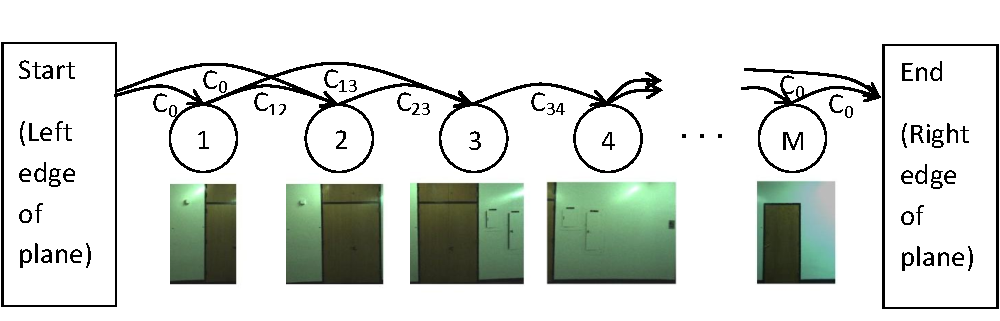
\includegraphics[width=3in]{dagCreation.pdf}
  \caption{DAG construction for the image selection process.}
  \label{fig:dagCreation}
\end{figure}

Figure \ref{fig:dagCreation} demonstrates the construction of a DAG
from overlapping images of a long hallway. Images are sorted by
horizontal location left to right, and become nodes in a
graph. Directed edges are placed in the graph from left to right
between images that overlap. The weights of these edges are determined
by the cost functions discussed previously. Next, we add two
artificial nodes, one start node representing the left border of the
plane, and one end node representing the right border of the
plane. The left artificial node has directed edges with equal cost
$C_0$ to all images that meet the left border of the plane, and the
right artificial node has directed edges from all images with that
meet the right border of the plane, with equal cost $C_0$ as well.

We now solve the standard shortest path problem from the start node to
the end node. This provides a set of images that completely covers the
plane horizontally, while minimizing the cost of the seams between
images.

In rare cases where the vertical dimension of the plane is not
entirely covered by a chosen image, we are left with a hole where no
image was chosen to texture. Rather than reverting to a 2D-coverage
problem, we can elect to simply fill the hole by selecting images to
fill it in a greedy fashion with respect to edge costs of the same
cost function.

With this completed, we have now mapped every location on our plane to
at least one image, and have minimized the amount of images, as well
as the discontinuity between their borders. In the next section, we
will apply blending between images where they overlap, but for the
sake of comparison with the unblended tile caching method in section
\ref{sec:mappingWithCaching}, we arbitrarily pick one image for
texturing where images overlap. Figure \ref{fig:compare_unblended}
compares the tile caching method against this seam minimization
method.

\begin{figure}
  \centering
  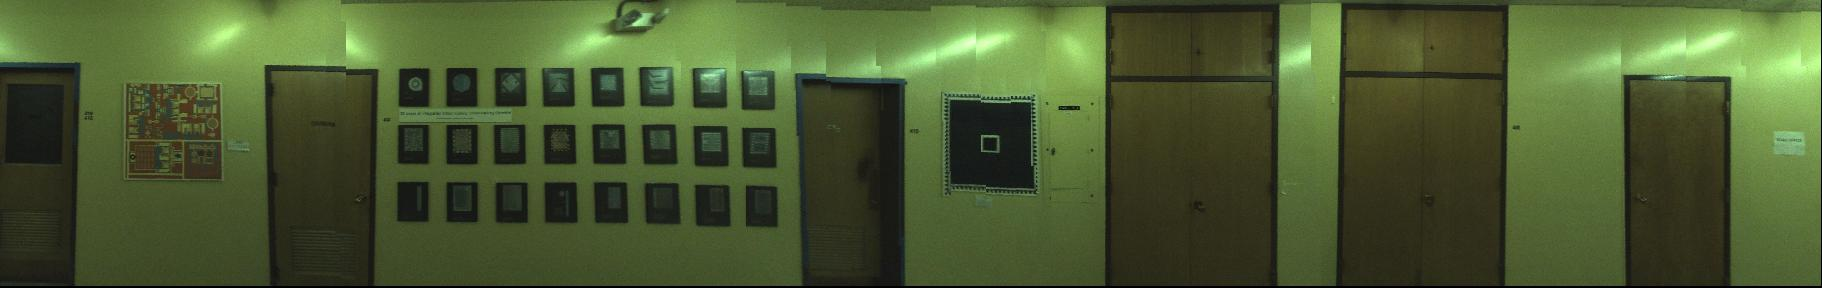
\includegraphics[width=3in]{wall1_cache_full_shifted.jpg}
  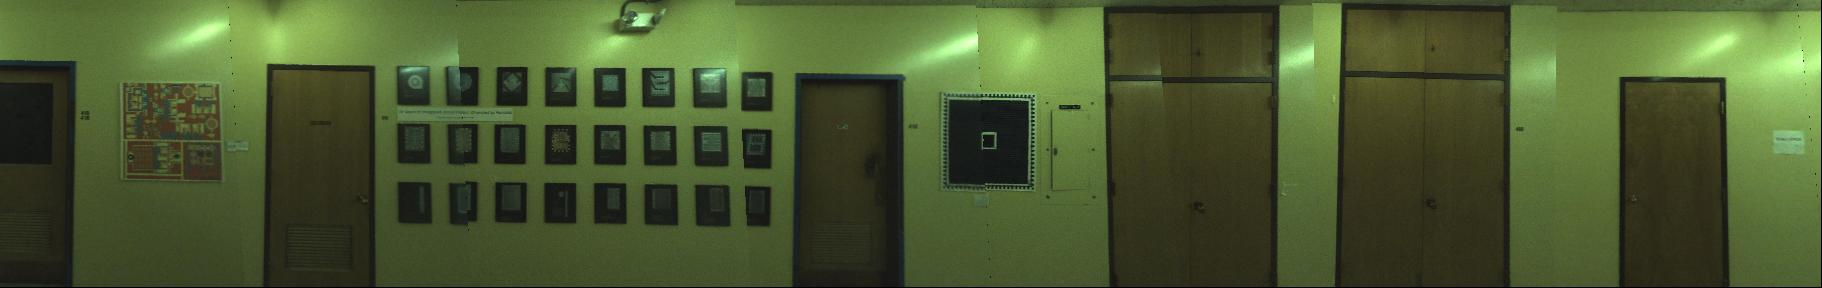
\includegraphics[width=3in]{wall1_dynprog_noblend.jpg}
  \caption{The tile caching approach is presented above the seam
    minimization approach.}
  \label{fig:compare_unblended}
\end{figure}


Though both methods provide quite accurate texturing thanks to the
localization refinement process, the seam minimization approach
results in fewer visible discontinuities, since it directly reduces
the cost of each image boundary, while the tile caching method uses a
scoring function that only approximates this effect. Furthermore, seam
minimization guarantees the best selection of images, while the tile
caching method may select images early on that turn out to be poor
choices once subsequent tiles have been processed.

In the context of the backpack modeling system, we apply the seam
minimization approach on walls, due to its superior output when
provided with optimal images. Floors and ceilings however, given their
suboptimal images, as shown in figure \ref{fig:floor_suboptimal}, can
only be textured using the tile caching method.

\subsection{Blending}
\label{sec:blending}
Until now, blending of images has not been used, for the sake of clear
comparisons between texturing methods. We will now apply the same
blending process on our two final texturing methods: localization
refinement followed by either tile caching or seam minimization.

Although our preprocessing steps and image selections in either method
attempt to minimize all mismatches between images, there are cases,
where due to different lighting conditions or inaccuracies in geometry
or projection, where we simply have unavoidable discontinuities. These
can however be treated and smoothed over by applying alpha blending
over image seams.  Whether the units we are blending are
rectangularly-cropped images or rectangular tiles, we can apply the
same blending procedure, as long as we have a guaranteed overlap
between units to blend over.

For the tile caching method, we can ensure overlap by texturing a
larger tile than we really have. For example, for a tile $l_1 x l_1$
in size, we can make sure to associate it with a texture $(l_1 + l_2)
x (l_1 + l_2)$ in size. For the seam minimization method, we have
already ensured overlap between images. To enforce consistent blending
however, it is beneficial to add a required overlap distance while
solving the shortest path problem in section
\ref{sec:imageSelection}. If images do not overlap in a region at
least the length of this overlap distance, we do not consider them to
overlap at all. If images overlap in a region greater than the overlap
distance, we will only apply blending over an area equal to the
overlap distance.

Our alpha blending technique is widely used, and blends pixels
linearly across overlapping regions. For each pixel within such a
region, we simply scale its intensity (by a factor from 0 to 1), based
on its distance from the image's border, with a cap set at a fixed
distance from the border. In this way, we interpolate between two
overlapping images, providing a gradual transition between them. Our
texture mapping process is now complete, and in figure
\ref{fig:pipeline}, we review our entire pipeline and demonstrate the
final blended output of both approaches.

\begin{figure}
  \centering
  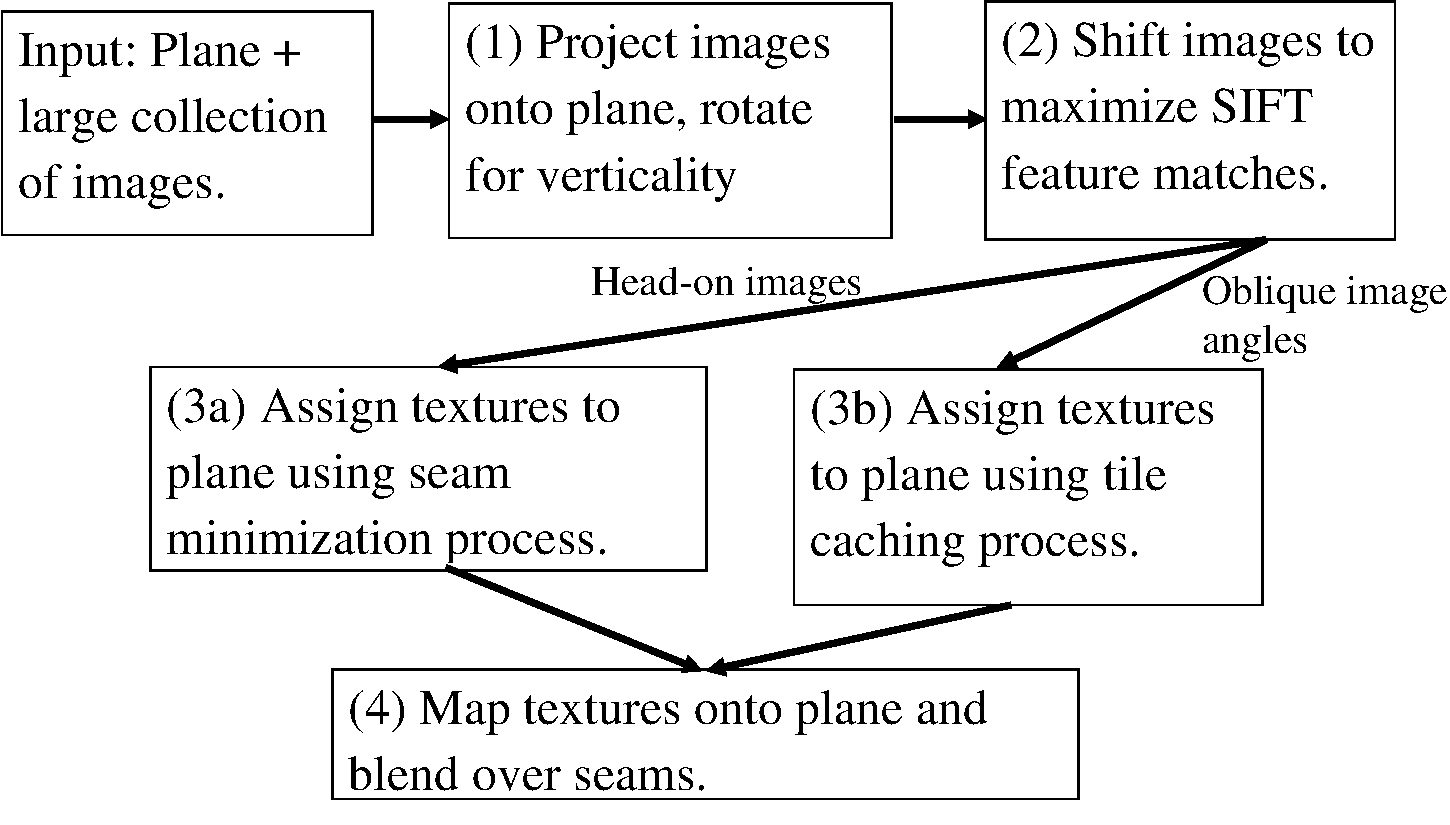
\includegraphics[width=3in]{pipeline.pdf}
  \caption{Our final texture processing pipeline, with the final
    output of both approaches.}
  \label{fig:pipeline}
\end{figure}


\section{Results and Conclusions}
\label{sec:resultsAndConclusions}
In this paper, we have shown how to accurately texture map models,
even when provided with imprecise camera localization data. We were
able to refine image locations based on feature mapping, and robustly
handle outliers.  We generalized one approach to texture mapping to
any manner of planes and images, and successfully textured both simple
rectangular walls as well as complex floor and ceiling geometry. We
also presented an optimized texturing method that takes advantage of
our localization refinement process and produces cleaner textures on
planes where multiple head-on images are available. Each of these
approaches is highly modular, and easily tunable for different
environments and acquisition hardware.

Ceilings and floors textured with the robust approach, and walls
textured with the optimized approach, are displayed in figure
\ref{fig:results}. A more detailed walkthrough demonstrating fully
textured 3D models using the approaches in this paper is available in
the accompanying video to this paper.

\begin{figure}
  \centering
  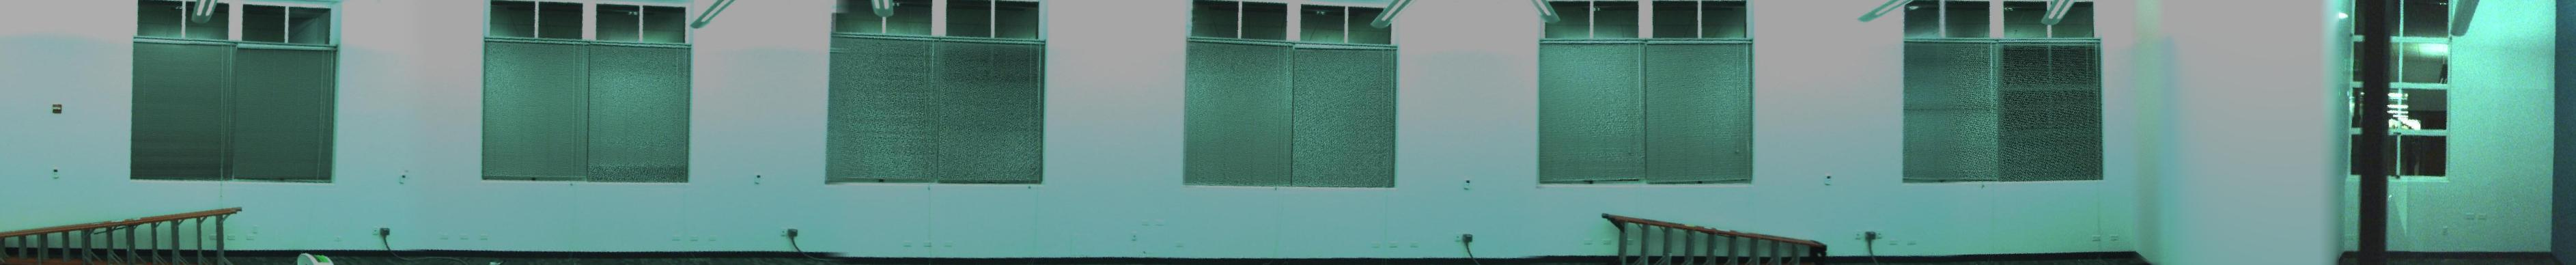
\includegraphics[width=3in]{4thfloor21.jpg}
  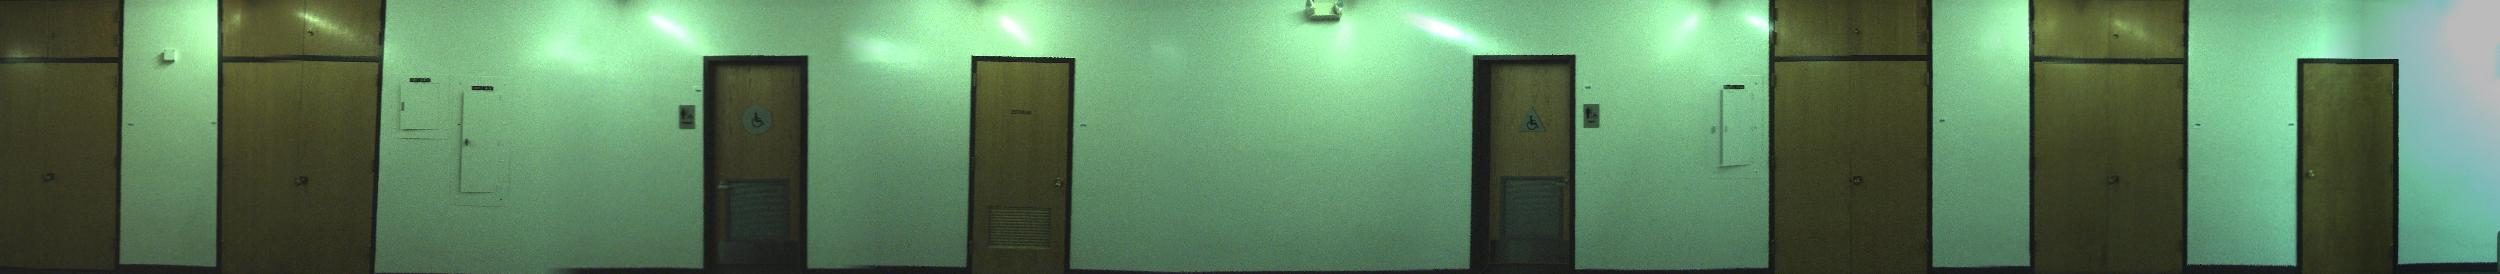
\includegraphics[width=3in]{4thfloor61.jpg}
  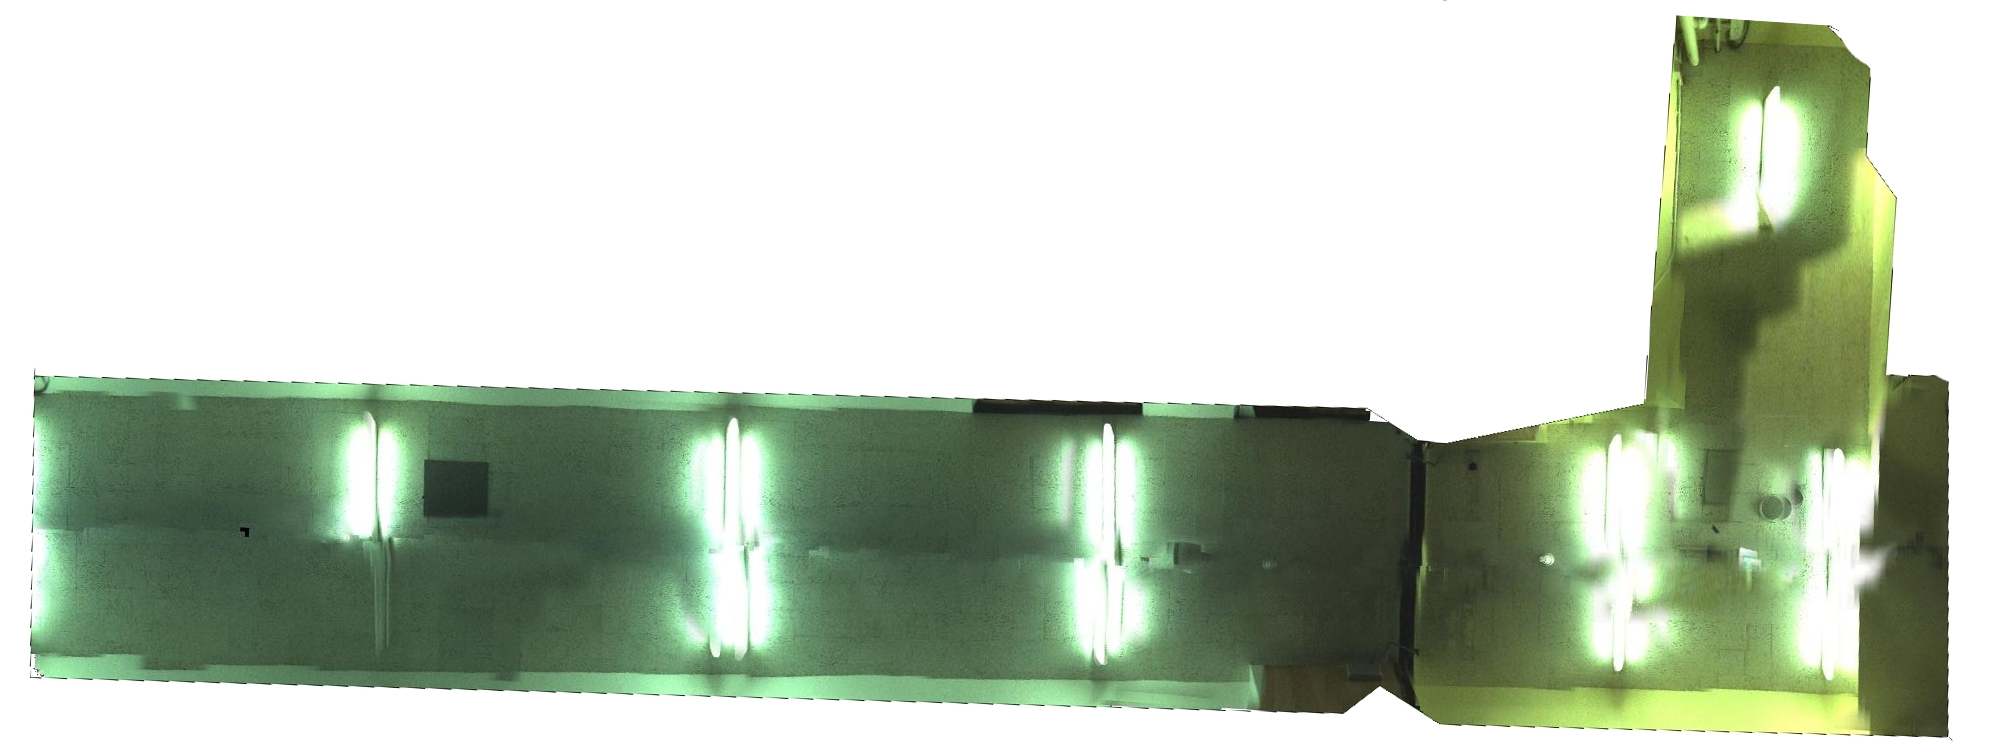
\includegraphics[width=2in]{4thfloor8.jpg}
  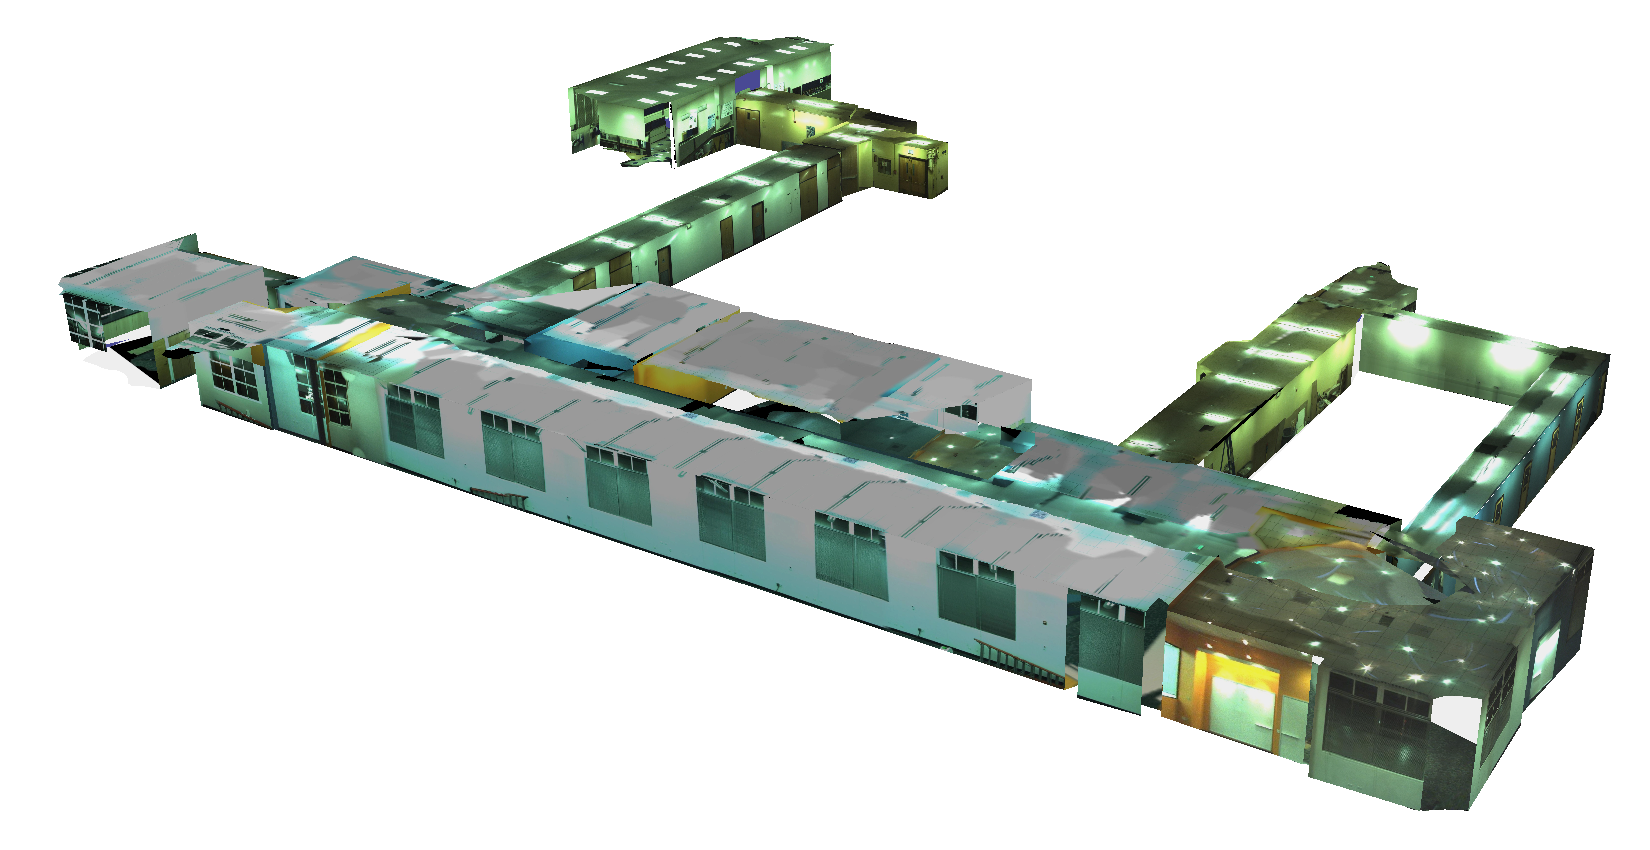
\includegraphics[width=3in]{fullmodel.png}
  \caption{Examples of our final texture mapping output for walls,
    floors, and ceilings}
  \label{fig:results}
\end{figure}

{\small \bibliographystyle{ieee} \bibliography{egbib} }


\end{document}
